\documentclass{beamer}
\usepackage{graphicx}
\usepackage{algorithm2e}
\usepackage{listings}
\usepackage{skak}
\usepackage{tikz}
\usetikzlibrary{graphdrawing,graphs,graphs.standard}
\usegdlibrary{trees}
\usepackage{forest}

\let\emptyset\varnothing

% \newrobustcmd*{\footlessfullcite}{\AtNextCite{\renewbibmacro{title}{}\renewbibmacro{in:}{}}\footfullcite}

\bibliography{docs}
\usetheme{Madrid}

\title{Turtles, Color, and Shapes}

% A subtitle is optional and this may be deleted
\subtitle{}

\author{James}
\institute{U. of West Georgia} \date{2015}

% Delete this, if you do not want the table of contents to pop up at
% the beginning of each subsection:
\AtBeginSubsection[]
{
  \begin{frame}<beamer>{Outline}
    \tableofcontents[currentsection,currentsubsection]
  \end{frame}
}

% Venn Diagram Circles
\def\firstcircle{(1,1) circle (0.5) (1,1.5)}
\def\secondcircle{(1.5,1) circle (0.5) (1.5,1.5)}
\def\containingrectablge{(0,0) rectangle (2.5, 2)}

\makeatletter
\pgfmathdeclarefunction{alpha}{1}{%
  \pgfmathint@{#1}%
  \edef\pgfmathresult{\pgffor@alpha{\pgfmathresult}}%
}

% Let's get started
\begin{document}

\begin{frame}
  \titlepage
\end{frame}

\begin{frame}{Outline}
  \tableofcontents
\end{frame}

\section{Code Website}

\begin{frame}[fragile]{Code Website}

All code presented in this talk is posted at this website.

\begin{verbatim}
https://github.com/jcchurch/PythonUCode/
\end{verbatim}

Adults: Go to this site for providing assistance.

\end{frame}

\section{Python}

\begin{frame}{What can you do with a computer?}

What can you do with a computer?

\pause

\begin{itemize}
\item Watch movies
\item Play games
\item Write stories
\item Make art
\item Browse the Internet
\pause
\item Do your homework!
\end{itemize}
\end{frame}

\begin{frame}{Computers}

Two key parts of a computer.

\begin{itemize}
\item Hardware (You can touch hardware.)
\item Software (It's inside the hardware.)
\end{itemize}
\end{frame}

\begin{frame}{Software}
\begin{itemize}
\item Programmers write software using a computer language.
\item Computers can only do what they are told.
\end{itemize}
\end{frame}

\begin{frame}{Why learn to code?}
\begin{itemize}
\item Coding is fun!
\item Coding is a valuable job skill.
\end{itemize}
\end{frame}

\begin{frame}{Python}
Look at these commands. What do you think they do? Using Python, try the following commands.
\begin{itemize}
\item 2 + 2
\item 7 + 3
\item 7 - 3
\item print('hello')
\item print('goodbye')
\end{itemize}
\end{frame}

\begin{frame}{Python Programming}
Let's write our first program!

To create a new program, click \textbf{File} and \textbf{New File}.
\end{frame}

\begin{frame}[fragile]{Our First Python Program}

\begin{verbatim}
name = input('What is your name?   ')
print('Hi, ', name)
\end{verbatim}

\begin{itemize}
\item To save a file, click \textbf{File} and \textbf{Save}. Save this program as \textbf{YourName1.py}. (If your name is Sarah, save this as \textbf{Sarah1.py})
\item To run your program, click \textbf{Run} and \textbf{Run Module}.
\end{itemize}
\end{frame}

\begin{frame}[fragile]{Change Your Program}

\begin{verbatim}
name = input('What is your name?   ')
print('Hi, ', name)
print('Hi, ', name)
print('Hi, ', name)
print('Hi, ', name)
\end{verbatim}

\begin{itemize}
\item To save a file, click \textbf{File} and \textbf{Save}. Save this program as \textbf{YourName2.py}. (If your name is Sarah, save this as \textbf{Sarah2.py})
\item To run your program, click \textbf{Run} and \textbf{Run Module}.
\end{itemize}
\end{frame}

\begin{frame}[fragile]{Change Your Program}

Let's change our program!

\begin{verbatim}
name = input('What is your name?   ')
print('Hi, ', name, name, name, name)
\end{verbatim}

\begin{itemize}
\item To save a file, click \textbf{File} and \textbf{Save}. Save this program as \textbf{YourName3.py}. (If your name is Sarah, save this as \textbf{Sarah3.py})
\item To run your program, click \textbf{Run} and \textbf{Run Module}.
\end{itemize}
\end{frame}

\begin{frame}[fragile]{MadLibs}

\begin{verbatim}
person = input('A person: ')
noun = input('A noun: ')
verb = input('A verb: ')
print('One day,',person,'went to a party.')
print('A big mean',noun,'stood in their way.')
print('So',person,'did a',verb,'and was able to get past!')
\end{verbatim}

Save this program as \textbf{MadLib.py}. Run it.
\end{frame}

\section{Turtles}

\begin{frame}{Turtles}
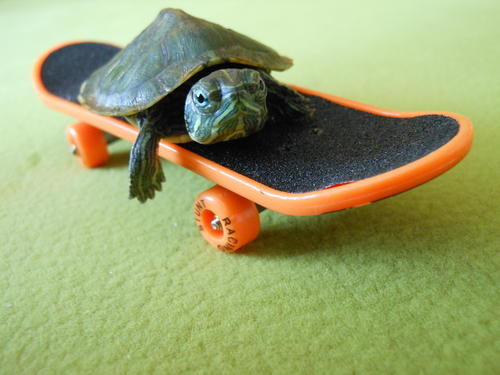
\includegraphics[width=70mm]{images/turtle_skateboard.jpg}
\end{frame}

\begin{frame}{Turtle Art}

\begin{itemize}
\item Turtles like to make art with their tail.
\item When their tail is down, they draw.
\item When their tail is up, the don't draw.
\end{itemize}

\end{frame}

\begin{frame}{Turtle Art}

\begin{itemize}
\item Turtles move forward.
\item Turtles turn left.
\item Turtles turn right.
\end{itemize}

\end{frame}

\begin{frame}[fragile]{Drawing with Turtles}

\begin{verbatim}
import turtle

window = turtle.Screen()

t = turtle.Turtle()
t.shape('turtle')
t.color('green', 'yellow')

t.down()
t.forward(100)

window.mainloop()
\end{verbatim}

Save this program as \textbf{MyTurtle1.py}. Run it.
\end{frame}

\begin{frame}{Turning}
\begin{itemize}
\item We want to draw a square.
\item The turtle must turn.
\item Turtles turn using degrees.
\item A corner turn is 90 degrees.
\end{itemize}

\end{frame}

\begin{frame}{Degrees}
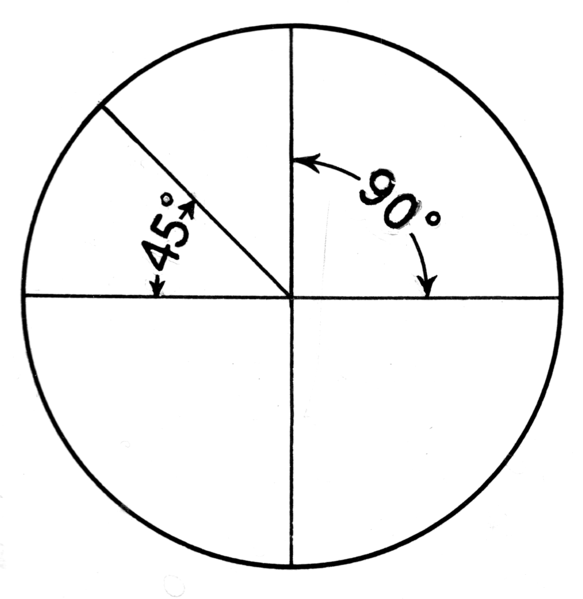
\includegraphics[width=70mm]{images/circle.png}
\end{frame}

\begin{frame}[fragile]{Drawing with Turtles}

Find the line in your code that says \textbf{t.forward(100)}. Add two lines after that line:

\begin{verbatim}
t.left(90)
t.forward(100)
\end{verbatim}

Save this program as \textbf{MyTurtle1.py}. Run it.
\end{frame}

\begin{frame}{Drawing the Square}

A square has 4 sides and 4 corners. How do we finish this program in order to make a square? Think-Write-Test-Repeat.

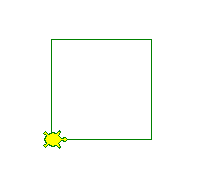
\includegraphics[width=50mm]{images/turtleSquare.png}

Once you've solved the problem, save this program as \textbf{MyTurtle1.py}. Run it.
\end{frame}

\begin{frame}[fragile]{Drawing the Square}

My solution

\begin{verbatim}
t.down()
t.forward(100)
t.left(90)
t.forward(100)
t.left(90)
t.forward(100)
t.left(90)
t.forward(100)
t.left(90)
\end{verbatim}

Save this program as \textbf{MyTurtle1.py}. Run it.
\end{frame}

\begin{frame}{Triangles}

Can we do triangles? Yes! It requires some math.

\begin{itemize}
\item There are three sides to a triangle.
\item There are three corners to a triangle.
\item In order to turn inward, we have to turn 90 degrees plus another 30 degrees.
\item What is 90 + 30?
\end{itemize}

\end{frame}

\begin{frame}[fragile]{Drawing a Triangle}

Make your program look like this again. Save this as \textbf{MyTurtle2.py}.

\begin{verbatim}
import turtle

window = turtle.Screen()

t = turtle.Turtle()
t.shape('turtle')
t.color('green', 'yellow')

t.down()
t.forward(100)

window.mainloop()
\end{verbatim}

\end{frame}

\begin{frame}{Drawing with Turtles}

A triangle has 3 sides and 3 corners. How do we finish this program in order to make a triangle?

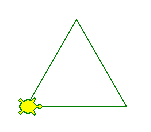
\includegraphics[width=50mm]{images/turtleTriangle.png}

Once you've solved the problem, save this program as \textbf{MyTurtle2.py}. Run it.
\end{frame}

\begin{frame}[fragile]{Drawing a Triangle}

My solution

\begin{verbatim}
t.down()
t.forward(100)
t.left(120)
t.forward(100)
t.left(120)
t.forward(100)
t.left(120)
\end{verbatim}
\end{frame}

\begin{frame}{Drawing a Square and a Triangle}

Challenge: Draw a square and a triangle in the same program.

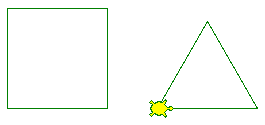
\includegraphics[width=50mm]{images/turtleSquareTriangle.png}

To do this, you'll need to draw the square, lift the turtle's tail using \textbf{t.up()}, move forward a distance of 150 units, then draw the triangle.

Once you've solved the problem, save this program as \textbf{MyTurtle3.py}. Run it.
\end{frame}

\begin{frame}{Draw Your Initial}

Let's spend some time playing with our turtles.

\begin{itemize}
\item Challenge: write your first initial using your turtle.
\item My first initial is J. I'm going to make my turtle draw a J.
\item Advice: This is going to be difficult. Think-Write-Test-Repeat
\begin{itemize}
\item Think about the turtle's next move.
\item Write that move.
\item Test your program. Did it make the move you wanted?
\item Repeat until finished.
\end{itemize}
\end{itemize}

\end{frame}

\section{Colors and Shapes}

\begin{frame}{Colors and Shapes}

This next phase will be extra challenging for our younger participants. Our youngest should continue working with turtles.

\end{frame}

\begin{frame}[fragile]{Colors and Shapes}
For our next part, we need to download a file to our programming folder.

\begin{verbatim}
http://bit.ly/PythonShapes
\end{verbatim}

Adults: I need your help downloading this file to everyone's computer. This file is called \textbf{shapes.py} on the code website.

\end{frame}

\begin{frame}{Horizontal and Vertical}

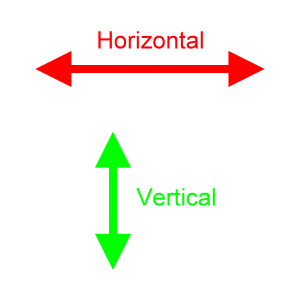
\includegraphics[width=50mm]{images/horizontalVertical.png}

\end{frame}

\begin{frame}{The Coordinate Plane}

\begin{itemize}
\item Everything on a window is at a coordinate.
\item A coordinate is a pair of numbers representing the horizontal distance and the vertical distance from the origin.
\item The top-left coordinate is called the origin. It's code is (0,0).
\item Every pixel is at a different coordinate. Horizontal first, vertical second.
\end{itemize}

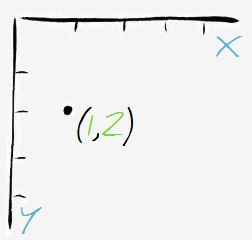
\includegraphics[width=50mm]{images/xyFlippedPlane.jpg}
\end{frame}

\begin{frame}[fragile]{Our First Shapes}

\begin{verbatim}
from shapes import *

window = createCanvas(600, 600)

drawRectangle(window, 25, 50, 125, 150, 'red')
drawCircle(window, 200, 100, 50, 'red')
drawTriangle(window, 325, 50, 100, 'red')

mainloop()
\end{verbatim}


Save this program as \textbf{MyShapes1.py}. Run it.

\end{frame}

\begin{frame}{Output of MyShapes1.py}
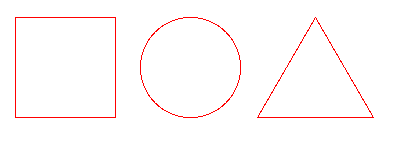
\includegraphics[width=50mm]{images/squareCircleTriangle.png}
\end{frame}

\begin{frame}[fragile]{Our First Shape: Rectangles}

\begin{verbatim}
drawRectangle(window, 25, 50, 125, 150, 'red')
\end{verbatim}

\begin{itemize}
\item 25: left horizontal
\item 50: top vertical
\item 125: right horizontal
\item 150: bottom vertical
\end{itemize}

There are two coordinates here: (25,50) and (125, 150). The computer can use these two coordinates to draw a shape.

\end{frame}

\begin{frame}[fragile]{Our First Shape: Circles}

\begin{verbatim}
drawCircle(window, 200, 100, 50, 'red')
\end{verbatim}

\begin{itemize}
\item 200: center horizontal
\item 100: center vertical
\item 50: radius
\end{itemize}

There is one coordinate: (200,100). The `50' is the size.

\end{frame}

\begin{frame}[fragile]{Our First Shape: Triangle}

\begin{verbatim}
drawTriangle(window, 325, 50, 100, 'red')
\end{verbatim}

\begin{itemize}
\item 325: top corner horizontal
\item 50: top corner vertical
\item 100: the height
\end{itemize}

There is one coordinate: (325,50). The 100 is the height!

\end{frame}

\begin{frame}[fragile]{Filled Shapes}

\begin{verbatim}
from shapes import *

window = createCanvas(600, 600)

drawFilledRectangle(window, 25, 50, 125, 150, 'red')
drawFilledCircle(window, 200, 100, 50, 'red')
drawFilledTriangle(window, 325, 50, 100, 'red')

mainloop()
\end{verbatim}


Save this program as \textbf{MyShapes2.py}. Run it.

\end{frame}

\begin{frame}{Output of MyShapes2.py}

\includegraphics[width=50mm]{images/squareCircleTriangleFilled.png}
\end{frame}

\begin{frame}[fragile]{Filled Shapes and Colors}

\begin{verbatim}
from shapes import *

window = createCanvas(600, 600)

drawFilledRectangle(window, 25, 50, 125, 150, 'orange')
drawFilledCircle(window, 200, 100, 50, 'blue')
drawFilledTriangle(window, 325, 50, 100, 'green')

mainloop()
\end{verbatim}

Save this program as \textbf{MyShapes3.py}. Run it.

\end{frame}

\begin{frame}{Output of MyShapes3.py}

\includegraphics[width=50mm]{images/squareCircleTriangleColors.png}

We can use these colors for our shapes: 'brown', 'white', 'black', 'red',
'green', 'blue', 'cyan', 'yellow', 'orange', and 'magenta'.

For some colors, you can add 'light' in front of a color, such as 'lightblue'.
\end{frame}

\begin{frame}{Play Time!}
For the rest of our UCode Session, we will play with the colors and shapes. Try making a picture of your house using rectangles, circles, and triangles.

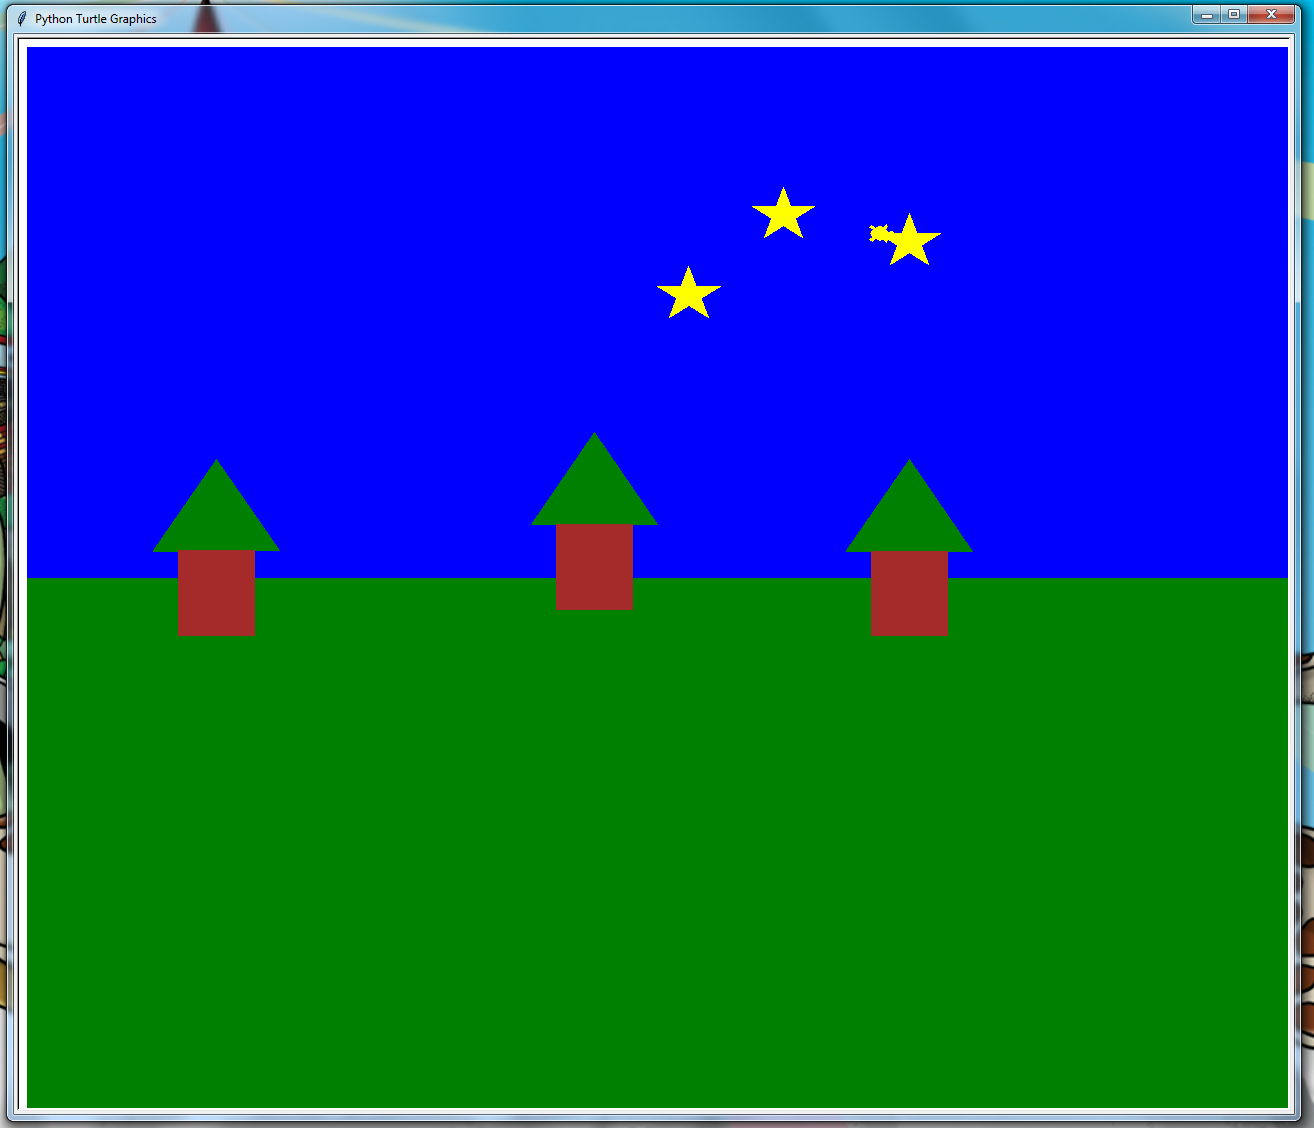
\includegraphics[width=50mm]{images/scene.png}
\end{frame}

\end{document}